\documentclass[a4paper,12pt]{report}

% ===================================================
% 1. PACKAGES & CONFIGURATION
% ===================================================
\usepackage[utf8]{inputenc}
\usepackage[english]{babel} 
\usepackage{geometry}      
\usepackage{titlesec}       
\usepackage{mathptmx}       
\usepackage{amsmath}
\usepackage{float}          
\usepackage[hidelinks]{hyperref}
\usepackage{array}         
\usepackage{caption}        
\usepackage{indentfirst}    
\usepackage{graphicx}
\usepackage[section]{placeins}
\usepackage{listings}
\usepackage{xcolor}
\usepackage{fancyhdr}
\usepackage{tikz}
\usetikzlibrary{calc}

% Page Margins (A4 Standard)
\geometry{
    top=2.5cm,
    bottom=2.5cm,
    left=3cm,
    right=2cm
}

% Configure page numbering in bottom right
\pagestyle{fancy}
\fancyhf{} % Clear all headers and footers
\fancyfoot[R]{\thepage} % Page number in bottom right
\renewcommand{\headrulewidth}{0pt} % Remove header line
\renewcommand{\footrulewidth}{0pt} % Remove footer line

% Redefine 'plain' style for Chapter pages to match
\fancypagestyle{plain}{
  \fancyhf{}
  \fancyfoot[R]{\thepage}
  \renewcommand{\headrulewidth}{0pt}
  \renewcommand{\footrulewidth}{0pt}
}

% Roman Numerals for Chapters (I, II, III...) like the sample
\renewcommand{\thechapter}{\Roman{chapter}}
\renewcommand{\thesection}{\arabic{section}}
\renewcommand{\thesubsection}{\thesection.\arabic{subsection}}

% Formatting Chapter Titles (e.g., Chapter I - Introduction)
\titleformat{\chapter}[display]
  {\normalfont\huge\bfseries\centering}
  {\chaptertitlename\ \thechapter}{10pt}{\Huge}
\titlespacing*{\chapter}{0pt}{-20pt}{30pt}

% ===================================================
% 2. STUDENT & PROJECT INFORMATION (EDIT HERE)
% ===================================================
\newcommand{\thesisTitle}{HanoiGO} % <--- Project Name
\newcommand{\thesisSubtitle}{Travel Planner for Hanoi}
\newcommand{\studentName}{Nguyen Duy Hung} % <--- Your Name
\newcommand{\studentID}{22BA13154}
\newcommand{\externalSupervisor}{Tran Thanh Tung}
\newcommand{\internalSupervisor}{Kieu Quoc Viet}
\newcommand{\reportDate}{Hanoi, June 2026}         % <--- Date
\setcounter{secnumdepth}{3}
\begin{document}

% ===================================================
% 3. COVER PAGE
% ===================================================
\newgeometry{left=2.5cm, right=2.5cm, top=2.5cm, bottom=2.5cm}
\begin{titlepage}
    \setlength{\parindent}{0pt}
    % Border around the page
    \begin{tikzpicture}[remember picture, overlay]
        \draw[line width = 1.5pt] ($(current page.north west) + (1.5cm,-1.5cm)$) rectangle ($(current page.south east) + (-1.5cm,1.5cm)$);
    \end{tikzpicture}
    
    \centering
    \vspace*{-0.7cm}
    
    % --- UNIVERSITY HEADER ---
    {\large \textbf{UNIVERSITY OF SCIENCE AND TECHNOLOGY OF HANOI}}\\[0.2cm]
    {\large \textbf{DEPARTMENT OF INFORMATION AND COMMUNICATION TECHNOLOGY}}\\[0.8cm]
    
    % --- LOGO ---
    \includegraphics[width=6.5cm]{logo-usth.png}\\[0.8cm]
    
    % --- THESIS TYPE ---
    {\fontsize{30pt}{36pt}\selectfont \textbf{BACHELOR THESIS}}\\[1cm]
    
    % --- AUTHOR ---
    {\large By}\\[0.2cm]
    {\large Nguyen Duy Hung}\\[0.1cm]
    {\large 22BA13154}\\[1cm]
    
    % --- TITLE ---
    {\large Title:}\\[0.2cm]
    {\fontsize{28pt}{34pt}\selectfont \textbf{HanoiGO - Travel Planner for Hanoi}}\\[1.8cm]
    
    % --- SUPERVISORS ---
    {\Large
    \renewcommand{\arraystretch}{1.3}
    \begin{tabular}{ll}
        External Supervisor: & Tran Thanh Tung \\
        Internal Supervisor: & Kieu Quoc Viet
    \end{tabular}}\\[0.5cm]
    
    \vfill
    
    % --- DATE ---
    {\large \textbf{Hanoi, June 2026}}\\[0.5cm]
\end{titlepage}
\restoregeometry

% ===================================================
% 4. CERTIFICATION OF RECOMMENDATION
% ===================================================
\newpage
\thispagestyle{plain}

\begin{center}
    To whom it may concern,
\end{center}

\vspace{1.5cm}

I, Kieu Quoc Viet (supervisor's name), certify that the thesis/ internship report of Mr. Nguyen Duy Hung (student's name) is qualified to be presented in the Internship Jury 2025-2026.

\vspace{4.5cm}

\hfill 
\begin{tabular}{c}
     Hanoi, June 2026 \\
     \textbf{Supervisor's signature}
\end{tabular}

% ===================================================
% 5. ACKNOWLEDGMENT
% ===================================================
\newpage
\thispagestyle{plain}
\begin{center}
    \Large \textbf{ACKNOWLEDGMENT}
\end{center}

\vspace{1cm}

{
\linespread{1.3}\selectfont
\setlength{\parskip}{1em}
\setlength{\parindent}{1.5em}

I would like to thank my supervisors, Kieu Quoc Viet and Tran Thanh Tung, for their support during the project. They provided useful comments and suggestions that helped me understand the problems more clearly. Their guidance encouraged me to think more carefully and improve my work step by step. They were always willing to answer my questions and give helpful advice when I faced difficulties. Thanks to their support, I was able to enhance the overall quality of the project.

\noindent Hanoi, June 2026
}

\vspace{3cm}

\noindent \textbf{Supervisor’s signature}

\newpage

% ===================================================
% 5. FRONT MATTER (TOC, LISTS)
% ===================================================
\pagenumbering{roman} % i, ii, iii...
{
\linespread{1.3}\selectfont
\setlength{\parskip}{0.5em}

\tableofcontents
\addcontentsline{toc}{chapter}{TABLE OF CONTENTS}
\newpage

\listoffigures
\addcontentsline{toc}{chapter}{LIST OF FIGURES}
\newpage

\listoftables
\addcontentsline{toc}{chapter}{LIST OF TABLES}
}
\newpage
% ===================================================
% 6. MAIN CONTENT
% ===================================================
\pagenumbering{arabic} % 1, 2, 3...

% --- CHAPTER I ---
\chapter{INTRODUCTION}

% Adjust spacing for Chapter I
\setlength{\parindent}{0pt} % No paragraph indentation
\setlength{\parskip}{1.2em} % Increase space between paragraphs
\linespread{1.3}\selectfont % Increase line spacing within paragraphs
\titlespacing*{\section}{0pt}{12pt}{4pt} % Reduce space after section headings

\section{Context}

Nowadays, more and more people travel abroad, and many of them use mobile phones or websites to plan their trips. According to Gretzel et al. \cite{gretzel2015smart}, using digital tools such as online maps and mobile apps can help tourists have a better travel experience. However, for foreign visitors who come to a big and crowded city like Hanoi \cite{vietnamtourism2024}, planning a trip on their own is often not easy, especially if they travel alone.

There are already some well-known travel apps like Google Maps, TripAdvisor, or Booking.com. But these apps usually only help with finding directions between two places. They are not built for planning a full trip across many days or for finding key information like place opening hours, local cultural tips, or descriptions in English. Because this kind of information is often scattered across many websites and blog posts, tourists have to spend a lot of time searching for it by themselves \cite{buhalis2020smartness}.

On top of that, solo travelers often have trouble finding other people to travel with, or splitting costs like taxi fares \cite{buhalis2019cocreation}. Most general social apps do not have a map feature, so it is hard to see if any group activity is happening nearby in real time. These issues make solo travel in Hanoi harder than it needs to be. There is a clear need for a simple and focused tool that puts maps, trip planning, and social features all in one place.

Because of this, I decided to build HanoiGO, a web application designed for foreign tourists visiting Hanoi. It helps users plan their daily trips automatically and connect with other travelers nearby on a shared map. The next section will explain in more detail why I decided to work on this project.

\section{Motivation}

The decision to undertake this project is driven by both practical travel navigation needs and technical aspirations.

First, I want to help tourists plan their trips more easily. I noticed that it is hard to arrange a list of tourist spots into a clear schedule across multiple days, especially because some places in Hanoi have specific opening hours or close for lunch. To solve this, I designed a multi-day scheduling method. It first groups tourist spots into daily clusters using K-Means clustering, and then finds a convenient order to visit places on each day using a Greedy Nearest Neighbor method that respects time limits. This scheduling method uses real-time travel times from the Goong Maps API to minimize waiting and travel time.

Second, I want to build a map-based feature that helps solo travelers meet other people. On most social networks, travel plans are shared only as text or photos, and there is no way to see where people are on a map. HanoiGO gives users a way to create and join group activities that are shown as dynamic markers on a live map. These markers change color and flash based on the activity's time status. When a user finds an interesting group activity, they can also copy the linked travel plan directly into their own account with a single click. This is done through a deep copy transaction in the database, which replicates all trip days and stops, and is much faster than re-creating the plan manually.

From a technical side, this project is also a chance for me to learn and practice useful development skills. I plan to use Next.js and TypeScript to build a responsive user interface, NestJS to build the backend server with a modular structure, PostgreSQL with PostGIS to store and query spatial location data, and WebSocket connections for real-time group chat.

With these motivations in mind, I established clear objectives to guide the development process.

\section{Objectives}

The main goal of this project is to build a complete web application that helps foreign tourists in Hanoi plan their trips and connect with other travelers more easily. To reach this goal, I have set a list of both functional and technical objectives.

In terms of features, I aim to do the following. First, I want to build a secure account system with email-based OTP verification so that only real users can access the platform. Second, I want to build a multi-day trip planner that automatically groups and sequences tourist spots into convenient daily plans using clustering and sequencing methods, taking into account real travel times, opening hours, and lunch breaks. Third, I aim to add a live map with dynamic status markers and a WebSocket-based group chat so travelers can easily find and communicate with other people nearby. Fourth, I plan to create a shared feed page with quick cloning features, allowing users to view, like, comment on, and instantly copy complete multi-day travel plans into their own account.

On the technical side, my goals are as follows. First, I will build a secure authentication system using stateless JWT tokens stored in HttpOnly cookies to protect against XSS attacks, combined with a token version field on each user account to allow token invalidation when needed. Second, I will use NestJS for the backend and Next.js for the frontend to create a clear and well-organized application. Third, I will use PostgreSQL with PostGIS extensions to store spatial location data and perform proximity queries efficiently. Fourth, I will implement real-time group messaging using WebSocket connections so that members of the same activity can communicate instantly in a shared chat room. Lastly, I will test and improve the scheduling algorithm to make sure it produces correct and useful results for a web application.

By reaching these goals, I hope to build something useful for foreign tourists in Hanoi and also show that I can apply modern web development skills in a real-world project.

% Reset spacing for subsequent chapters
\setlength{\parindent}{15pt}
\setlength{\parskip}{0em}
\linespread{1}\selectfont

% --- CHAPTER II ---
\chapter{SYSTEM ANALYSIS}

% Apply same spacing as Chapter I
\setlength{\parindent}{0pt}
\setlength{\parskip}{0.6em}
\linespread{1.3}\selectfont
\titlespacing*{\section}{0pt}{12pt}{4pt}

\section{Overview}

This chapter explains how the system works internally, showing the main features, the key modules, and how different components interact with each other. It describes how the ideas introduced in Chapter I are turned into a working web application.
 
HanoiGO is designed for two types of users: Tourists and Administrators. Tourists use the platform to explore places in Hanoi, generate daily trip schedules automatically, and join group activities on a live map. Administrators manage user accounts and keep the platform running smoothly through a dedicated management panel.
 
The system is built using a modern technology stack. The backend is developed with NestJS, and the frontend is built with Next.js. Location data is stored and queried using PostgreSQL with the PostGIS extension. Real-time group chat is handled through WebSocket connections using Socket.io. This architecture helps the system manage different types of data efficiently and respond quickly to user actions.

\section{System Requirements}

Overall, the HanoiGO application for helping foreign tourists plan and enjoy their trips in Hanoi has to satisfy the following main requirements:
 
\begin{itemize}
    \item For Tourists:
    \begin{itemize}
        \item Register and log in securely with email-based identity verification.
        \item Browse and filter tourist places in Hanoi on an interactive map.
        \item Generate multi-day trip schedules automatically based on selected places and travel preferences.
        \item Create and join group activities displayed on the map.
        \item Communicate with other travelers using real-time group chat.
        \item Share and clone trip plans through a social feed.
        \item Manage personal profiles and saved trip itineraries.
        \item Report activities that violate platform guidelines.
    \end{itemize}
 
    \item For Administrators:
    \begin{itemize}
        \item View a dashboard showing platform statistics and system reports.
        \item Manage user accounts, including searching, blocking, and deleting users.
        \item Manage tourist place information and coordinates.
        \item Manage and moderate group activities on the map.
        \item Review and resolve violation reports submitted by users.
    \end{itemize}
\end{itemize}

\section{UML Diagrams}

This section presents the Use Case diagrams to visualize the interactions between the actors and the system.

\subsection{Use Case Diagram}

\subsubsection{Tourist Use Case}

Figure~\ref{fig:usecase_tourist} shows how tourists interact with the HanoiGO system. They can perform operations across five core sub-systems: Authentication, Profile Management, Places Discovery, Trip Planning, and Activity Management. The main access points are directly connected to the Tourist actor, while specialized operations are connected via standard UML include and extend relationships. This structure allows tourists to easily transition from exploring places to planning schedules, hosting activities on the map, and communicating in group chats.

\begin{figure}[H]
    \centering
    \includegraphics[width=1\linewidth]{user-usecase.drawio.pdf} 
    \caption{Use Case Diagram for Tourist}
    \label{fig:usecase_tourist}
\end{figure}

\newpage
\begin{table}[H]
\centering
\small
\renewcommand{\arraystretch}{1.1}
\begin{tabular}{|c|p{4.5cm}|p{9cm}|}
\hline
\textbf{No.} & \textbf{Use Case} & \textbf{Description} \\ \hline
1 & Login & Access the platform using credentials. \\ \hline
2 & Register & Create an account, extending the Login process. \\ \hline
3 & Manage Profile & Access personal profile management. \\ \hline
4 & View Profile & View profile details, extending Manage Profile. \\ \hline
5 & Update Profile & Edit user details and language, extending Manage Profile. \\ \hline
6 & Change Password & Update account password, extending View Profile. \\ \hline
7 & Browse Places & Explore cultural and historical landmarks. \\ \hline
8 & View Place List & View list of registered places, included in Browse Places. \\ \hline
9 & View Place Detail & See description and coordinates, extending Browse Places. \\ \hline
10 & Like Places & Bookmark landmarks to basket, extending View Place List. \\ \hline
11 & Plan Trip & Access itinerary planning and scheduling. \\ \hline
12 & Generate Trip & Calculate optimized daily routes, extending Plan Trip. \\ \hline
13 & Save Trip & Save computed schedule to profile, extending Generate Trip. \\ \hline
14 & View My Trips & Browse saved itineraries, extending Plan Trip. \\ \hline
15 & Delete Trip & Permanently remove a saved trip, extending View My Trips. \\ \hline
16 & Share Saved Trip & Start activity from saved trip, extending View My Trips. \\ \hline
17 & Manage Activities & Access activity hosting and joining options. \\ \hline
18 & Host Activity & Access hosting features, extending Manage Activities. \\ \hline
19 & CRUD Activity & Create, update, and delete activities, included in Host Activity. \\ \hline
20 & Manage Join Requests & Approve or reject participant requests, extending Host Activity. \\ \hline
21 & Join Activity & Request to join another group, extending Manage Activities. \\ \hline
22 & Browse Activities & View active events on the map, included in Manage Activities. \\ \hline
23 & Report Activities & Flag an activity for violations, extending Browse Activities. \\ \hline
24 & Chat Group & Send real-time messages in group, extending Host Activity and Join Activity. \\ \hline
\end{tabular}
\caption{Descriptions of Tourist Use Cases}
\label{tab:tourist_use_cases}
\end{table}

\subsubsection{Admin Use Case}

Figure~\ref{fig:usecase_admin} outlines the administrative functions provided by the HanoiGO platform. The Admin actor manages the system through five main sub-systems: Dashboard, User Management, Place Management, Activity Management, and Report Management. The primary administrative features are directly linked to the Admin actor, while secondary actions are connected using standard UML include and extend relationships. This modular design helps the administrator monitor platform activities, moderate content, update landmark information, and maintain a safe community environment.

\begin{figure}[H]
    \centering
    \includegraphics[width=1\linewidth]{admin-usecase.drawio.pdf} 
    \caption{Use Case Diagram for Admin}
    \label{fig:usecase_admin}
\end{figure}

\newpage
\begin{table}[H]
\centering
\small
\renewcommand{\arraystretch}{1.1}
\begin{tabular}{|c|p{4.5cm}|p{9cm}|}
\hline
\textbf{No.} & \textbf{Use Case} & \textbf{Description} \\ \hline
1 & View Dashboard & Access the administrative dashboard to monitor the platform. \\ \hline
2 & View Statistics & Monitor user activity and system metrics, included in View Dashboard. \\ \hline
3 & Manage Users & Access account management and user administration features. \\ \hline
4 & View User List & Browse all registered accounts in the system, included in Manage Users. \\ \hline
5 & Block User & Restrict platform access for accounts that violate guidelines, extending View User List. \\ \hline
6 & Unblock User & Restore access for previously restricted user accounts, extending View User List. \\ \hline
7 & Delete User & Permanently remove a user account from the database, extending View User List. \\ \hline
8 & View User Detail & Inspect detailed profile information and activity logs of a user, extending Manage Users. \\ \hline
9 & Create User & Add new user or administrator accounts manually, extending Manage Users. \\ \hline
10 & Manage Places & Access landmark and geographical location management tools. \\ \hline
11 & View Place List & Browse all registered tourist landmarks in Hanoi, included in Manage Places. \\ \hline
12 & Update Place & Edit descriptions, categories, or opening hours of a place, extending View Place List. \\ \hline
13 & Delete Place & Permanently remove a landmark entry from the database, extending View Place List. \\ \hline
14 & Create Place & Add new landmarks with GPS coordinates and spatial data, extending Manage Places. \\ \hline
15 & Manage Activities & Access activity moderation and administration tools. \\ \hline
16 & View Activities List & Browse all active group activities on the map, included in Manage Activities. \\ \hline
17 & Manage Reports & Access system moderation and community safety tools. \\ \hline
18 & Review Reports & Inspect complaints and violation flags submitted by users, included in Manage Reports. \\ \hline
19 & Handle Reports & Resolve reported violations and take disciplinary actions, extending Review Reports and Manage Activities. \\ \hline
\end{tabular}
\caption{Descriptions of Admin Use Cases}
\label{tab:admin_use_cases}
\end{table}

\subsection{Sequence Diagrams}

This subsection shows sequence diagrams that explain step-by-step interactions in the HanoiGO system. They illustrate how components work together for key functions like user authentication, trip planning, and group activity management. 

Figure~\ref{fig:seq_login} shows the steps of the login process. The user enters their email and password, which are sent to the backend for verification. The backend checks the database to find the account and compares the password. If the login fails, an error message is displayed to the user; if it is successful, the backend generates a JWT access token and redirects the user to the discovery page.

\begin{figure}[H]
    \centering
    \includegraphics[width=0.95\linewidth]{login-seq.png}
    \caption{Sequence Diagram for Login flow}
    \label{fig:seq_login}
\end{figure}

Figure~\ref{fig:seq_plan_trip} shows how the system generates and saves a multi-day trip plan. The user selects places on the map and sets trip parameters such as the number of days, travel date, and start and end times. The backend fetches the selected places, removes closed ones, groups them into daily clusters using K-Means, and calls the Goong Maps API to get travel times. A Greedy Nearest Neighbor algorithm then builds the daily routes, and any dropped places are re-inserted where possible. When the user confirms the result, the frontend saves the full trip structure to the database.

\begin{figure}[H]
    \centering
    \includegraphics[width=0.95\linewidth]{plantrip-seq.png}
    \caption{Sequence Diagram for Plan Trip flow}
    \label{fig:seq_plan_trip}
\end{figure}

Figure~\ref{fig:seq_activity} shows three related sub-flows for the Activity feature. In the Browse flow, the frontend fetches nearby activities using a PostGIS proximity query and displays them as status-coded markers on the map. In the Host flow, the user fills in the activity form and the backend saves the activity with a geospatial point and adds the creator as an approved member; the host can also approve or reject join requests, which updates the member status and notifies the requester. In the Join flow, a user sends a join request that is stored as a pending member record and a notification is sent to the host.

\begin{figure}[H]
    \centering
    \includegraphics[width=0.95\linewidth]{activity-seq.png}
    \caption{Sequence Diagram for Activity flow}
    \label{fig:seq_activity}
\end{figure}

Figure~\ref{fig:seq_group_chat} shows the real-time group chat flow. In the Connect flow, the frontend opens a connection to the \texttt{/group-chat} namespace using a JWT token. After verification, the gateway joins the user to the room, loads the last 30 messages, and sends the online users list. In the Send Message flow, the frontend displays the message optimistically and emits it to the gateway, which saves it to the database and broadcasts it to all sockets in the room.

\begin{figure}[H]
    \centering
    \includegraphics[width=0.85\linewidth]{chat-seq.png}
    \caption{Sequence Diagram for Group Chat flow}
    \label{fig:seq_group_chat}
\end{figure}

\newpage
% Reset spacing for Chapter III and subsequent sections
\setlength{\parindent}{15pt}
\setlength{\parskip}{0em}
\linespread{1}\selectfont

% --- CHAPTER III ---
\chapter{METHODOLOGY}

% Apply same spacing as Chapter II
\setlength{\parindent}{0pt}
\setlength{\parskip}{0.6em}
\linespread{1.3}\selectfont
\titlespacing*{\section}{0pt}{12pt}{4pt}

This chapter describes the high-level architecture of HanoiGO, detailing the frontend navigation, modular NestJS backend structure, and the integration of PostgreSQL/PostGIS databases. It also formulates the mathematical logic and heuristics used for K-Means++ clustering and the Travelling Salesman Problem with Time Windows (TSPTW).

\section{System Architecture}

This section presents the system architecture to give an overview of how the HanoiGO platform is structured. Figure~\ref{fig:sys_arch} presents the system architecture of HanoiGO, which is designed in a client--server model. The system includes four main components: Client Layer, Core Backend, Data Layer, and External Services.

\begin{figure}[H]
    \centering
    \makebox[\textwidth][c]{\includegraphics[width=1.25\textwidth]{sys-arc.pdf}}
    \caption{HanoiGO System Architecture Diagram}
    \label{fig:sys_arch}
\end{figure}

The Client Layer is the web interface used by travelers. It is built with Next.js and TypeScript to ensure stable performance. This layer communicates with the backend using HTTP for normal actions and WebSocket for real-time features such as group chat and notifications.

The Core Backend is responsible for handling the main functions of the system. It manages user authentication using JWT and Passport. The backend includes several modules, such as user management, admin functions, trip planning, activities, and notification handling. Prisma ORM is used to interact with the database, while Socket.io supports real-time communication.

The Data Layer stores system data using PostgreSQL. PostgreSQL with the PostGIS extension is used for structured data, geographical information, and spatial queries. Redis is also configured in the environment to support future chat scaling. This design helps the system work efficiently with different types of data.

The External Services component includes third-party services that support the platform. The Goong Maps API is used to calculate travel times and distance matrices. SMTP via Gmail is used for sending verification emails, while Supabase Storage handles uploaded media files.

\section{Tools and Techniques}

This section describes the main development tools and approaches used to build the platform.

\subsection{Development Tools}

Visual Studio Code was used as the main code editor for its TypeScript support. Git with GitHub managed version control, and pull requests were reviewed before merging. Docker ran the PostgreSQL and Redis services in containers to keep the setup consistent across machines. For the database, Prisma defined the schema and managed migrations, generating the matching SQL commands automatically when the schema changed.

\subsection{Frontend Techniques}

The frontend is built with Next.js, using the App Router to manage routes and loading states. It separates Server Components, rendered on the server, from Client Components that handle user interactions, which helps pages load faster. The Socket.io Client connects to the backend over WebSockets for real-time group chat and notifications, while React Hooks (including custom hooks for authentication and socket management) handle component state. The interface uses Tailwind CSS so it adapts to different screen sizes, from desktops to smartphones.

\subsection{Backend Techniques}

The backend is built with NestJS, which organizes code into modules such as authentication, group chat, and trip planning. Each module has controllers for incoming requests and services for the business logic. Real-time features use NestJS WebSocket gateways, which verify the JWT token on connection and place users into rooms by activity ID so messages reach only the correct members. File uploads use Multer middleware, which limits uploads to image files up to 10MB and stores them in Supabase Storage with a local storage fallback.

\section{Backend Development}
\subsection{Authentication}

The system utilizes JSON Web Tokens (JWT) to manage user identity and access control. Upon a successful login, a token containing the user's ID, username, and role (USER or ADMIN) is generated. For security purposes, these tokens are digitally signed and valid for 7 days. They are primarily stored in browser cookies (via HttpOnly cookies), with a backup in the authorization headers for WebSocket stability. While public routes like registration are accessible to all, private features such as Group Chat and Trip Planning are restricted through role-based access control (RBAC).

To ensure data integrity, passwords are encrypted using the bcrypt hashing algorithm, making them irreversible even if the database is compromised. Additionally, a security verification policy is implemented: user accounts require entering a six-digit OTP code sent via Gmail before registration is complete to prevent spam accounts.

The password complexity requirements are summarized in Table~\ref{tab:password_rules}:

\begin{table}[H]
\centering
\begin{tabular}{|p{4cm}|p{9cm}|}
\hline
\textbf{Rule} & \textbf{Description} \\
\hline
Minimum length & At least 8 characters \\
\hline
Uppercase letter & Must include A--Z \\
\hline
Lowercase letter & Must include a--z \\
\hline
Number & Must include 0--9 \\
\hline
Special character & Must include symbols like !@\#\$\%\^{}\&* \\
\hline
\end{tabular}
\caption{Password Requirements}
\label{tab:password_rules}
\end{table}

These requirements ensure that passwords are complex enough to resist common attacks. If a password doesn't meet all the rules, the system shows an error message and asks the user to create a stronger password.

\subsection{Trip Planner}

The trip planner is the core feature of HanoiGO. It builds convenient multi-day itineraries from a set of selected places, the number of travel days, and the daily start and end times. The planner handles both spatial data (where the places are) and temporal constraints (opening hours, lunch breaks, and the daily time limit). 

To solve this problem efficiently for a web application, the system implements a multi-stage heuristic pipeline. The sequence of these planning stages is illustrated in Figure~\ref{fig:trip_pipeline}. The process consists of five sequential steps:

\begin{figure}[H]
    \centering
    \includegraphics[width=0.6\linewidth]{trip-pipeline.png}
    \caption{The multi-stage trip planning pipeline of HanoiGO}
    \label{fig:trip_pipeline}
\end{figure}

\textbf{Step 1: Pre-Filtering} 
\\ The system first checks the selected places against the user's travel dates. Any place that is closed on all days of the trip is filtered out. This pre-filtering step ensures that subsequent clustering and sequencing steps do not waste resources on unreachable places.

\textbf{Step 2: Geographic Clustering with Capacity Limits} 
\\ The remaining places are grouped into $K$ clusters (where $K$ is the number of travel days) using the K-Means++ clustering method. The objective is to minimize the total geographic spread within each day, which is calculated using the sum of squared distances:
\[
J = \sum_{c=1}^{K} \sum_{p \in C_c} d_{\text{Haversine}}(p, \mu_c)^2
\]
where $C_c$ is the set of places assigned to day $c$, and $\mu_c$ is the centroid of that day's cluster. 

Since clustering only requires relative proximity, it uses the straight-line distance calculated offline via the Haversine formula to maintain fast performance:
\[
d_{\text{Haversine}}(i, j) = 2 R \arcsin \left( \sqrt{\sin^2\left(\frac{\Delta \phi}{2}\right) + \cos(\phi_i) \cos(\phi_j) \sin^2\left(\frac{\Delta \lambda}{2}\right)} \right)
\]
where $R$ is the Earth's radius (6371 km). 

After clustering, the system applies two adjustments:
\begin{itemize}
    \item \textbf{Capacity Rebalancing:} Each daily cluster is capped at a maximum of 5 places to keep the schedule realistic. If a cluster exceeds this limit, the place furthest from the centroid is moved, where possible, to the geographically closest cluster that has available capacity.
    \item \textbf{Closed-Day Swapping:} If a place in a cluster is closed on that specific day of the week, the system attempts to swap it to another day's cluster where it is open and where capacity is available.
\end{itemize}

\textbf{Step 3: Distance Matrix Prefetching and Fallbacks}
\\ To sequence the daily routes, the system needs real-world road travel durations instead of straight-line distances. The primary source is the Goong Maps Distance Matrix API. To reduce the number of API calls, for trips with up to $N \le 24$ places the system prefetches all durations in a single query: from the user's starting point to every place, and between every pair of places. Each entry is the motorbike travel duration in seconds:
\[
t(i, j) = \text{GoongMatrix}(i, j)
\]
When querying travel durations, the system attempts up to three retries with exponential backoff if the Goong API is rate-limited. If the query still fails, it falls back to estimating travel times from the Haversine distance and the average motorbike speed $v_{\text{avg}}$ (30 km/h):
\[
t_{\text{travel}}^{\text{fallback}}(i, j) = \frac{d_{\text{Haversine}}(i, j)}{v_{\text{avg}}} \times 3600
\]

\textbf{Step 4: Route Sequencing and Time Window Checking}
\\ For each day, the system sequences the places using a Greedy Nearest Neighbor (GNN) heuristic to solve the Travelling Salesman Problem with Time Windows (TSPTW). 

If a starting location is provided, the algorithm starts at the place closest to the traveler's starting location; otherwise, it begins at the first available open location. It then repeatedly selects the next stop that minimizes a transition cost. The transition cost penalizes travel time over waiting time to keep the route compact:
\[
\text{Cost}(i, j) = t_{\text{travel}}(i, j) \times 2 + t_{\text{wait}}(j)
\]
where $t_{\text{travel}}(i, j)$ is the motorbike travel time in seconds, and $t_{\text{wait}}(j)$ is the time in seconds the traveler waits if they arrive before place $j$ opens. 

During sequencing, the system tracks the arrival time, wait time, and departure time at each stop. The arrival time $T_{\text{arrive}}(j)$ at a stop includes travel time and a 10-minute parking and entry buffer. If the arrival time overlaps with the lunch break (defaulting to 11:00--13:00), the arrival is shifted to after lunch. The wait time is defined as:
\[
t_{\text{wait}}(j) = \max(0, T_{\text{open}}(j) - T_{\text{arrive}}(j))
\]
and the departure time at place $j$ is calculated as:
\[
T_{\text{depart}}(j) = \max(T_{\text{arrive}}(j), T_{\text{open}}(j)) + t_{\text{visit}}(j)
\]
A stop is scheduled only if its visit finishes before both its own closing time and the daily end time; otherwise, the stop is dropped from the initial greedy route and handled later in the cascade and conflict resolution stages. The planner also reports the remaining free time at the end of each day (calculated as the difference between the daily end time and the last departure time) so users can see if more stops can be added.

\textbf{Step 5: GPS Cascade and Conflict Resolution}
\\ Once the initial sequence is created, the system performs a final validation:
\begin{itemize}
    \item \textbf{GPS Coordinate Cascade:} The actual travel time from the user's starting location to the first stop is injected. This shifts the arrival and departure times of all subsequent stops. If a stop violates the closing time or daily end time, it is dropped from the schedule. The travel time between its predecessor and successor is then recomputed, and the time shifts are cascaded down the remaining stops.
    \item \textbf{Gap Insertion:} Any places dropped during the clustering, sequencing, or cascade phases are passed to a conflict resolution stage. The system attempts to insert these dropped places back into "gaps" (between scheduled stops) of any day where the place is open, provided it fits within its time window and does not make subsequent stops infeasible.
\end{itemize}
The parameter values used in these steps are summarized in Table~\ref{tab:trip_parameters}.

\begin{table}[h!]
\centering
\caption{Trip Planner Parameter Specifications}
\label{tab:trip_parameters}
\renewcommand{\arraystretch}{1.3}
\begin{tabular}{|p{2.8cm}|p{2.5cm}|p{5.5cm}|p{3.7cm}|}
\hline
\textbf{Parameter} & \textbf{Default} & \textbf{Value Representation} & \textbf{Core Role} \\ \hline
Avg Speed & 30 km/h & Average speed for motorbikes & Travel time fallback \\ \hline
Earth Radius & 6371 km & Constant for sphere geometry & Distance calculation \\ \hline
Parking Buffer & 10 min & Time added per stop & Parking and entry buffer \\ \hline
Lunch Break & 11:00--13:00 & Time block in minutes from midnight (user-configurable) & Blocked window for breaks \\ \hline
\end{tabular}
\end{table}

\subsection{Activity}

The Activity module is a key social feature of HanoiGO. It enables solo travelers to host group activities on a map, connect with other travelers, and share trip plans. The module is organized around three main functions, summarized in Table~\ref{tab:activity_functions}.

\begin{table}[H]
\centering
\small
\renewcommand{\arraystretch}{1.2}
\begin{tabular}{|>{\raggedright\arraybackslash}p{4cm}|>{\raggedright\arraybackslash}p{9.5cm}|}
\hline
\textbf{Function} & \textbf{Description} \\ \hline
Activity Hosting and Map Browsing & Store activity locations as PostGIS geometry points; display all open activities on a Leaflet.js map with status-coded markers; show the user's current location as a reference point. \\ \hline
Membership and Join Requests & Submit and manage join requests with a daily rate limit; approval or rejection saves a notification to the database and emits a real-time Socket.io event to the member; users can report violations. \\ \hline
Transactional Itinerary Replication & Clone the trip linked to an activity into the user's profile in a single atomic database operation. \\ \hline
\end{tabular}
\caption{Activity Module Functions}
\label{tab:activity_functions}
\end{table}

\textbf{Activity Hosting and Map Browsing}
\\ To host a new activity, the user defines its details (such as the title, category, and scheduled time) and sets the location. The coordinates can be entered directly or derived from the first stop of a linked trip. The backend stores this location as a PostGIS geometry point in the WGS84 coordinate system (SRID 4326), and the host is automatically added as the first approved member. On the frontend, a Leaflet.js map displays all open activities that the user has not yet joined, drawn as color-coded markers. Each marker's status is derived on the client from the scheduled time relative to the current time, giving four states: upcoming, starting soon (within 2 hours of the start), ongoing (from the start time up to 3 hours after), and ended. If the user grants location permission, their current position is also shown on the map as a reference point.

\textbf{Membership and Join Requests}
\\ Travelers can submit a join request to any open activity. The member record follows a defined state lifecycle, shown in Table~\ref{tab:member_states}. Each user is limited to at most 5 join requests per day to prevent misuse. Users can also report an activity for guideline violations; each report stores the reporter, reason, and optional evidence for administrator review.

\begin{table}[H]
\centering
\small
\renewcommand{\arraystretch}{1.2}
\begin{tabular}{|p{2.5cm}|p{4cm}|p{2.5cm}|p{4.5cm}|}
\hline
\textbf{From State} & \textbf{Trigger} & \textbf{To State} & \textbf{Side Effect} \\ \hline
--- & User submits request & \texttt{PENDING} & Notify host \\ \hline
\texttt{PENDING} & Host approves & \texttt{APPROVED} & Notify member \\ \hline
\texttt{PENDING} & Host declines & \texttt{REJECTED} & Notify member \\ \hline
\texttt{PENDING} & User cancels & (deleted) & --- \\ \hline
\end{tabular}
\caption{Member Status State Transitions}
\label{tab:member_states}
\end{table}

\textbf{Transactional Itinerary Replication}
\\ To make sharing plans convenient, travelers can copy the multi-day trip linked to an activity into their own profile with a single click. The backend replicates the entire trip structure (including all days and stops) in a single Prisma nested write, which is automatically executed as an atomic database operation. After the trip is saved, the activity's save count is incremented in a separate update.

\subsection{Group Chat}

The Group Chat module enables real-time communication between approved activity members. The system uses a WebSocket gateway to manage connections, message delivery, and user presence.

\textbf{Real-Time Gateway and Presence Management}
\\ Members communicate through a NestJS WebSocket gateway under the \texttt{group-chat} namespace. When a client connects, the gateway verifies the JWT token from the handshake before any messaging is allowed. The client then emits a \texttt{join\_activity} event, and only after the gateway confirms the user is an approved member does it place the client into a dedicated room named \texttt{activity\_\{activityId\}}. Online presence and typing indicators are tracked using two in-memory hash maps (\texttt{onlineMap} and \texttt{typingMap}), with a 3-second auto-stop for typing. Redis is configured in the environment for future scaling, but the current implementation runs on a single server. \\

\textbf{Message Persistence and Offline Dispatch}
\\ When a message is sent, the backend saves it to PostgreSQL and broadcasts it to the room at the same time. Messages and emoji reactions are stored in the \texttt{Message} and \texttt{MessageReaction} tables, keeping all chat data in one database. After broadcasting, the server checks which approved members are not currently in the room and creates a database notification for each of them, with a short summary of the message (for example, a text preview or a note that an image or file was sent). This process is shown in Figure~\ref{fig:chat_pipeline}. \\

\textbf{File Attachments and Read Tracking}
\\ Besides plain text, the module also supports image and file attachments. Each message has a \texttt{type} field (\texttt{TEXT}, \texttt{IMAGE}, or \texttt{FILE}), and attachment messages additionally store the \texttt{mediaUrl}, \texttt{fileName}, and \texttt{fileSize}. The files themselves are uploaded through a separate REST endpoint and saved to Supabase Storage, with a local-disk fallback when the storage service is not configured.

To show unread message counts, the system keeps a \texttt{MessageReadStatus} record for each user and activity that stores the last read time. When a user opens a room, the gateway returns the recent messages together with an unread count computed from messages created after that time, excluding the user's own messages. A \texttt{mark\_read} event then updates the last read time when the user views the room.

\begin{figure}[H]
    \centering
    \includegraphics[width=1\linewidth]{chat-pipeline.png}
    \caption{Real-time Group Chat Pipeline}
    \label{fig:chat_pipeline}
\end{figure} 

The main events used in the Group Chat module are summarized in Table~\ref{tab:chat_events}.

\begin{table}[H]
\centering
\small
\renewcommand{\arraystretch}{1.2}
\begin{tabular}{|p{3.8cm}|p{3cm}|p{6.7cm}|}
\hline
\textbf{Event Name} & \textbf{Direction} & \textbf{Description} \\ \hline
\texttt{join\_activity} & Client $\rightarrow$ Server & Verify APPROVED membership, join room \texttt{activity\_\{id\}}, and load message history. \\ \hline
\texttt{message\_history} & Server $\rightarrow$ Client & Send the most recent 30 messages and the unread message count when the chat is opened. \\ \hline
\texttt{mark\_read} & Client $\rightarrow$ Server & Update the last read time for the current user when the room is viewed. \\ \hline
\texttt{load\_more\_messages} /~\texttt{more\_messages} & Client $\leftrightarrow$ Server & Request and deliver an older page of messages for pagination. \\ \hline
\texttt{send\_message} & Client $\rightarrow$ Server & Send a new text, image, or file message to be stored and broadcast. \\ \hline
\texttt{new\_message} & Server $\rightarrow$ Client & Deliver a new message to all members in the room. \\ \hline
\texttt{react\_message} /~\texttt{message\_reacted} & Client $\leftrightarrow$ Server & Toggle an emoji reaction and broadcast the updated reactions. \\ \hline
\texttt{typing} /~\texttt{stop\_typing} & Client $\rightarrow$ Server & Indicate whether a user is typing, with a 3-second auto-stop. \\ \hline
\texttt{typing\_users} /~\texttt{online\_users} & Server $\rightarrow$ Client & Update the typing indicator and the online presence list. \\ \hline
\end{tabular}
\caption{Socket.io Group Chat Events}
\label{tab:chat_events}
\end{table}

These events support the core functionalities required for real-time group communication.

\subsection{Moderation System}

The moderation system supports community safety by allowing tourists to report guideline violations and providing administrators with tools to review those reports and act on users or group activities.

Tourists report a group activity or user profile by selecting a violation type (such as spam, scam, or hate speech) and writing a brief description; the report is created with a \texttt{PENDING} status. From a dedicated dashboard, administrators review pending reports and either dismiss a report (marking it \texttt{DISMISSED} with no further action) or resolve it (marking it \texttt{RESOLVED} and optionally hiding the reported activity by setting its status to \texttt{CANCELLED}, or deleting it). Administrators can also suspend user accounts directly.

On the backend, when an administrator decides to suspend an account, the controller triggers the \texttt{banUser} method in \texttt{AdminService}. The database operation runs inside a transaction block to update the user status, increment the token version, create a resolved report, and log the action. The steps executed during account suspension are summarized in Table~\ref{tab:ban_process}:

\begin{table}[H]
\centering
\begin{tabular}{|c|p{3.5cm}|p{9.5cm}|}
\hline
\textbf{Step} & \textbf{Action} & \textbf{Description} \\ \hline
1 & Database Status & Change the user status to \texttt{BANNED} in the database. \\ \hline
2 & Token Invalidation & Increment the \texttt{tokenVersion} to immediately invalidate active JWT sessions on subsequent requests. \\ \hline
3 & Action Audit & Create a resolved report entry and record the action details in the \texttt{AdminLog} table. \\ \hline
4 & Notification & Dispatch an \texttt{ADMIN\_WARNING} notification informing the user of the account suspension. \\ \hline
\end{tabular}
\caption{Steps Executed During User Suspension}
\label{tab:ban_process}
\end{table}

On the frontend, the admin panel is built with Next.js using dynamic routing for detailed report views and dashboard widgets. Admin views include statistical breakdowns of violations, user search tables with action buttons, and moderation queues with status badges.

Each moderation action runs inside a Prisma transaction, so the related writes either all succeed or all roll back, avoiding partial updates. Every action, including suspending or restoring a user, resolving or dismissing a report, and cancelling or deleting an activity, is recorded in the \texttt{AdminLog} table to provide an audit trail. Role-based access control (RBAC) via the \texttt{RolesGuard} decorator restricts moderation endpoints to users with the \texttt{ADMIN} role, and JWT token versioning revokes a suspended user's access instantly without a stateful token blacklist.

A key limitation of the current moderation system is its reliance on manual reports by users rather than automated content filtering. Future enhancements will explore integrating natural language processing to automatically flag inappropriate content before it is published.

\section{Frontend Development}

The frontend is built with Next.js and the App Router. To keep the project organized, pages are grouped into three route groups by audience and access level, as summarized in Table~\ref{tab:route_groups}. The \texttt{(auth)} group holds the public sign-in pages, the \texttt{(main)} group holds the tourist-facing pages, and the \texttt{admin} group holds the moderation panel. The role stored in the JWT is read in \texttt{middleware.ts} to send each user to the correct group after login.

\begin{table}[H]
\centering
\small
\renewcommand{\arraystretch}{1.2}
\begin{tabular}{|p{2.5cm}|p{5.5cm}|p{5cm}|}
\hline
\textbf{Route Group} & \textbf{Main Pages} & \textbf{Purpose} \\ \hline
\texttt{(auth)} & login, register, verify-email, forgot-password, reset-password & Public account and OTP flows. \\ \hline
\texttt{(main)} & discovery, places/[id], trips, activities, profile & Tourist features behind login. \\ \hline
\texttt{admin} & dashboard, users, places, activities, reports & Moderation panel for the \texttt{ADMIN} role. \\ \hline
\end{tabular}
\caption{Frontend Route Groups and Pages}
\label{tab:route_groups}
\end{table}

Inside the \texttt{(main)} group, a fixed \texttt{Header} gives access to the core pages: Discovery, Trips, Activities, and Places. The header navigation also shows badges for saved places and the total number of unread group-chat messages so users notice new activity without opening each page.

\begin{figure}[H]
    \centering
    \makebox[\textwidth][c]{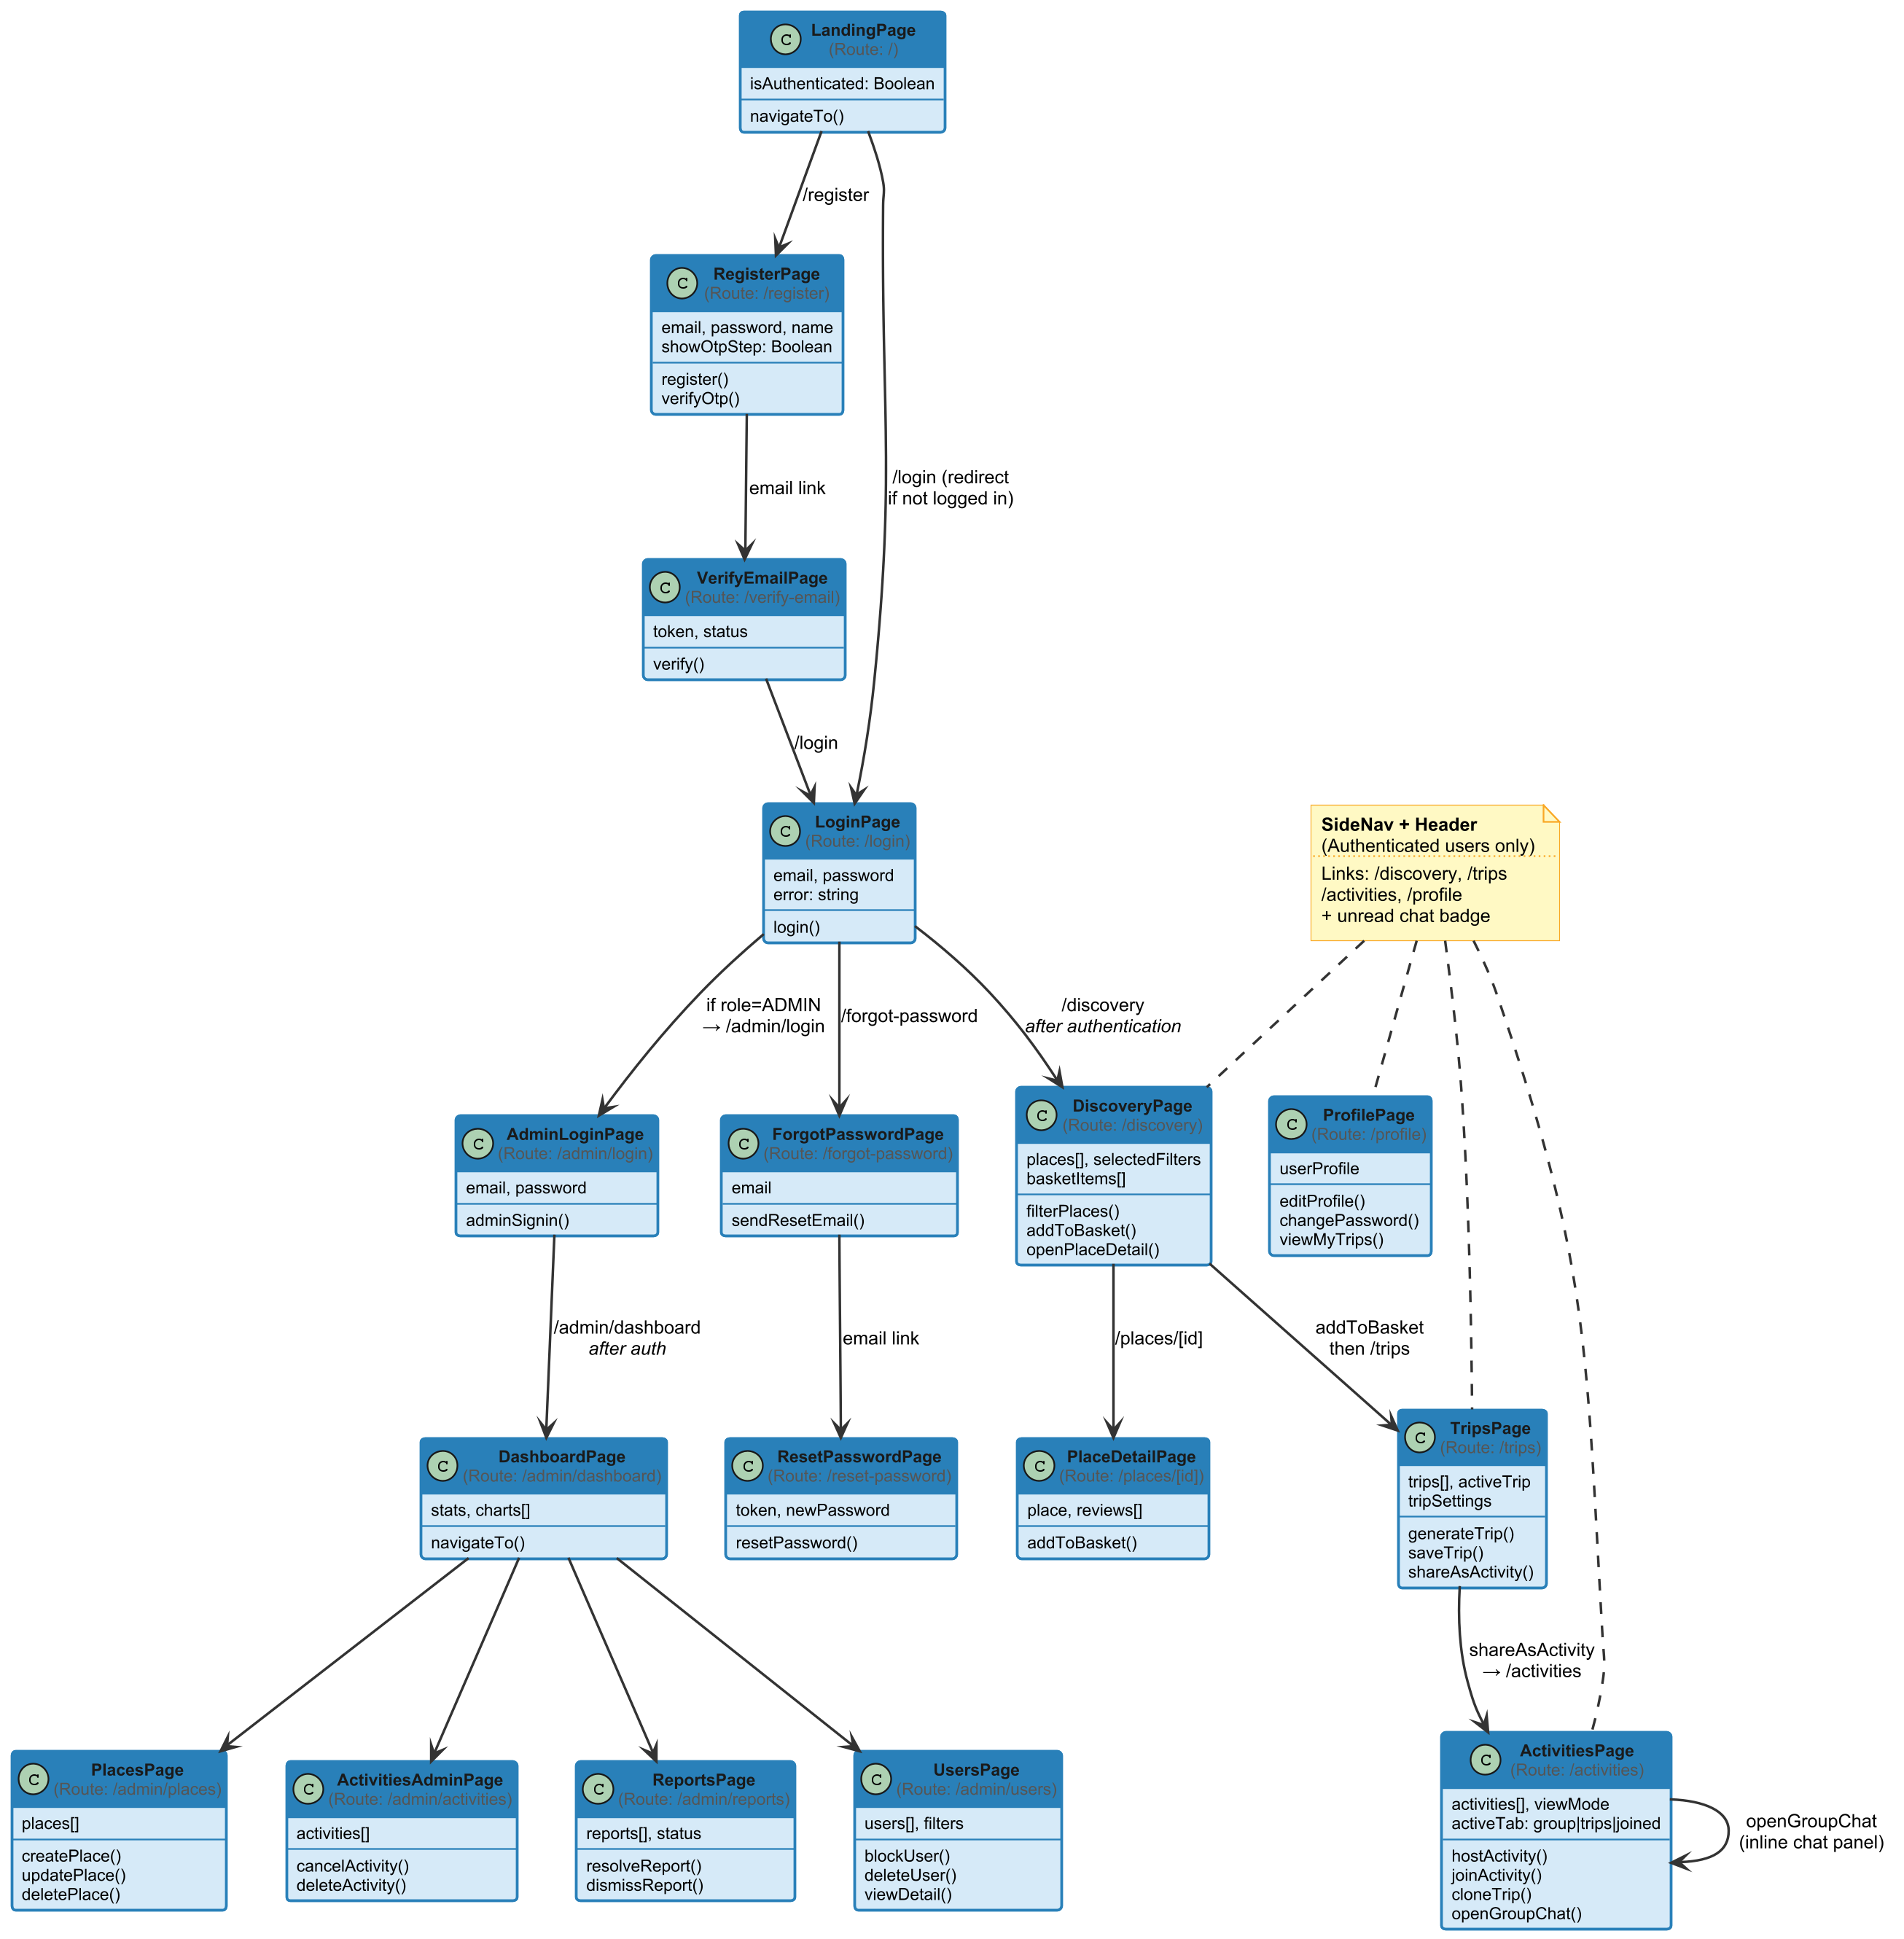
\includegraphics[width=1.2\textwidth]{navigation-diagram.pdf}}
    \caption{HanoiGO Frontend Navigation Diagram}
    \label{fig:nav_diagram}
\end{figure}

\subsection{UI Design System}

The interface is styled with Tailwind CSS using custom semantic tokens defined in \texttt{globals.css} and \texttt{tailwind.config}, so colors and spacing stay consistent across pages. The palette uses a rose primary color (\texttt{\#FF5A5F}) on a warm champagne surface, the Manrope font, and Material Symbols icons. The main technologies and their roles are listed in Table~\ref{tab:frontend_tech}.

\begin{table}[H]
\centering
\small
\renewcommand{\arraystretch}{1.2}
\begin{tabular}{|p{3.5cm}|p{10cm}|}
\hline
\textbf{Technology} & \textbf{Role in the Frontend} \\ \hline
Next.js (App Router) & Page routing, Server and Client Components, and loading states. \\ \hline
Tailwind CSS & Utility-first styling with shared semantic color tokens. \\ \hline
Leaflet.js & Interactive maps for discovery, trip routes, and activities. \\ \hline
Socket.io Client & Real-time group chat and notification updates. \\ \hline
Zustand & Lightweight client-side state stores. \\ \hline
Recharts & Charts on the admin dashboard. \\ \hline
\end{tabular}
\caption{Main Frontend Technologies}
\label{tab:frontend_tech}
\end{table}

All map components are loaded with \texttt{next/dynamic} and \texttt{ssr: false}. This is required because Leaflet uses the browser \texttt{window} object, which is not available during server-side rendering and would otherwise cause an error.

\subsection{Client-Side State with Zustand}

Shared state is kept in small Zustand stores instead of one global object, so each feature only reads what it needs. The main stores are listed in Table~\ref{tab:zustand_stores}. The trip basket is saved to \texttt{sessionStorage}, which lets a user keep their selected places while moving between the Discovery and Trips pages, but clears the selection when the tab is closed.

\begin{table}[H]
\centering
\small
\renewcommand{\arraystretch}{1.2}
\begin{tabular}{|p{4.5cm}|p{6.0cm}|p{2.8cm}|}
\hline
\textbf{Store} & \textbf{Responsibility} & \textbf{Persistence} \\ \hline
\texttt{use\allowbreak Auth\allowbreak Store} & Current user and session state. & \texttt{local\allowbreak Storage} \\ \hline
\texttt{use\allowbreak Trip\allowbreak Store} & Selected places (basket) and trip settings. & \texttt{session\allowbreak Storage} \\ \hline
\texttt{use\allowbreak Chat\allowbreak Notification\allowbreak Store} & Unread message count per activity. & In-memory \\ \hline
\texttt{use\allowbreak Notification\allowbreak Store} & Toast messages for user feedback. & In-memory \\ \hline
\texttt{use\allowbreak Confirm\allowbreak Store} & Shared confirmation dialog state. & In-memory \\ \hline
\end{tabular}
\caption{Zustand State Stores}
\label{tab:zustand_stores}
\end{table}

\subsection{Places Discovery and Trip Planner Interface}

On the Discovery page, tourists browse landmarks on a Leaflet map and add the ones they like to a travel basket. The basket is shown as a floating widget (\texttt{TravelBasket}) that stacks the selected place thumbnails and links to the planner. When the user opens the Trips page, a settings modal collects the trip parameters (number of days, daily start and end time, lunch break, visit duration, travel date, and start location). The start location can be the user's current position or a custom place searched through Goong Maps autocomplete.

After the schedule is generated, the planner uses a two-panel layout (see Figure~\ref{fig:trip_planner_ui}). The left panel is a timeline of stops grouped by color-coded day tabs, and the right panel is the map showing the route. Selecting a day tab filters the map to that day only, and the day colors match the markers so the timeline and the map stay easy to read together. From this view, the user can save the trip or share it as a group activity.

\subsection{Activity and Live Map Interface}

The Activities page has two view modes (a card feed and a map) and three tabs that separate plain group activities, shared trips, and the activities the user has joined. On the map, each activity is drawn as a marker whose color and animation are computed on the client from the scheduled time, so the map reflects the live status without reloading. The four marker states are listed in Table~\ref{tab:marker_states}, and the activity map interface is detailed in Figure~\ref{fig:activity_map_ui}.

\begin{table}[H]
\centering
\small
\renewcommand{\arraystretch}{1.2}
\begin{tabular}{|p{2.8cm}|p{2.5cm}|p{3.5cm}|p{3.7cm}|}
\hline
\textbf{Status} & \textbf{Color} & \textbf{Visual Cue} & \textbf{Time Condition} \\ \hline
Upcoming & Blue & Static marker & More than 2 hours before start \\ \hline
Starting soon & Amber & ``SOON'' badge & Within 2 hours of start \\ \hline
Ongoing & Green & Pulsing ``LIVE'' badge & Start time up to 3 hours after \\ \hline
Ended & Gray & Faded marker & More than 3 hours after start \\ \hline
\end{tabular}
\caption{Live Activity Marker States}
\label{tab:marker_states}
\end{table}

When a user opens an activity that is linked to a trip, the interface offers a single button to clone that trip into their own profile, which avoids copying the plan by hand. Markers also show the host name and member count in a popup before the user decides to view or join.

\subsection{Group Chat Interface}

Approved members chat inside the activity view through the \texttt{ActivityChat} component, which connects to the WebSocket gateway using \texttt{ChatSocketProvider}. To make the chat feel responsive, a sent message appears immediately in the user's own view before the server confirms it (optimistic rendering). The interface also shows typing indicators, supports emoji reactions, and marks messages as read when the room is open. Unread counts are kept in \texttt{useChatNotificationStore} and surfaced both on the activity tab and on the side navigation badge, so a user can see new messages from anywhere in the application.

\subsection{Admin Dashboard and Moderation UI}

The admin panel is built with the same Next.js stack and uses Recharts for its charts, since Recharts works with React and resizes to fit different screen sizes. The dashboard opens with summary cards for active users, heritage sites, total trips, and pending reports, followed by charts for user growth, violation types, report status, and popular places. The other admin pages reuse a common table layout with status badges and action buttons for managing users, places, activities, and reports (see Figure~\ref{fig:admin_dashboard_ui}).

\section{Database Design}

The database system of HanoiGO is built on PostgreSQL, a common relational database management system, with the PostGIS extension enabled to support geospatial operations. The database schema is defined and managed using the Prisma Object-Relational Mapping (\texttt{Prisma ORM}) tool, which provides type safety and manages database migrations. PostgreSQL is selected because it is a stable relational database that handles structured application data efficiently. The PostGIS extension is chosen because it adds support for geographic objects, allowing the application to run location-based queries like finding nearby places and activities. Prisma is used to simplify database interactions and to ensure consistency between the application source code and the database tables. One trade-off of this setup is that running location queries on a single-node database is sufficient for the current scope of HanoiGO, but a larger system would require dedicated spatial index optimizations or distributed replicas to handle heavy traffic.

The complete database schema contains 15 application tables and is illustrated in Figure~\ref{fig:db_complete}. The schema is organized into three main functional clusters: identity and system administration; places and trip planning; and activity and group chat. Each cluster is described below alongside a diagram of the tables it contains.

\begin{figure}[H]
    \centering
    \makebox[\textwidth][c]{\includegraphics[width=1.25\textwidth]{HanoiGO_Diagram_2.pdf}}
    \caption{HanoiGO Database Schema Diagram}
    \label{fig:db_complete}
\end{figure}


\subsection{Identity and System Administration}

This cluster manages identity, account status, administrative accountability, content safety, and user notifications. By combining these security and feedback mechanisms, the system isolates user account lifecycle events and administrative oversight from the public geographic features. It contains four tables.

\begin{itemize}
    \item \texttt{users}: The central table of the system. It stores login credentials (\texttt{password\_hash}), profile fields (\texttt{username}, \texttt{full\_name}, \texttt{nationality}, \texttt{languages}), role assignment (\texttt{role}: \texttt{USER} or \texttt{ADMIN}), and account lifecycle state (\texttt{status}: \texttt{ACTIVE}, \texttt{PENDING}, or \texttt{BANNED}). The \texttt{token\_version} field is used to invalidate all existing JWT tokens for a user when the account is banned or when the user resets their password. The \texttt{otp\_code} and \texttt{otp\_expires\_at} fields support the email-based password reset flow.

    \item \texttt{reports}: Records user-submitted complaints against other users or specific content items (activities, messages). The \texttt{entity\_type} and \texttt{entity\_id} fields allow a single table to reference any reportable object. An admin resolves each report by setting \texttt{status} to \texttt{RESOLVED} or \texttt{DISMISSED} and optionally adding \texttt{admin\_notes}.

    \item \texttt{admin\_logs}: A permanent audit trail of every administrative action. Each row links an admin user (\texttt{admin\_id}), the action string, and an optional \texttt{target\_id}. This table is append-only in practice; no delete operation is exposed through the API.

    \item \texttt{notifications}: Stores in-app notifications delivered to users after key events, such as a join request being approved (\texttt{ACTIVITY\_APPROVED}) or a new message arriving (\texttt{NEW\_MESSAGE}). The \texttt{entity\_type} and \texttt{entity\_id} fields allow the frontend to link the notification to the relevant page. The \texttt{is\_read} boolean is updated when the user opens the notification panel. Two indexes, on \texttt{(user\_id, is\_read)} and \texttt{(user\_id, created\_at)}, support the common queries for fetching unread counts and ordered notification history.
\end{itemize}

\begin{figure}[H]
    \centering
    \makebox[\textwidth][c]{\includegraphics[width=1.25\textwidth]{db-identity-admin.pdf}}
    \caption{Database Cluster: Identity and System Administration}
    \label{fig:db_identity_admin}
\end{figure}

\subsection{Places and Trip Planning}

This cluster stores geographical data and the structured output of the trip planner algorithm. It is the most spatially aware part of the schema.

\begin{itemize}
    \item \texttt{places}: Each row represents a tourist landmark in Hanoi. The \texttt{location} column stores a PostGIS \texttt{geometry(Point, 4326)} value, which enables the \texttt{ST\_DWithin} proximity query used by the discovery feature. The opening hours are stored as separate fields (\texttt{open\_days} as an integer array, \texttt{open\_time\_start}, \texttt{open\_time\_end}) so the trip planner can check time-window feasibility when sequencing stops. A GiST index on the \texttt{location} column is defined to keep spatial queries fast.

    \item \texttt{place\_gallery}: Stores additional image URLs linked to a place. It is kept separate from the \texttt{places} table to avoid widening the main row and to allow cascade deletion when a place is removed.

    \item \texttt{trips}: Each trip belongs to one user and has a \texttt{num\_days} value set at generation time. The \texttt{cloned\_from\_id} self-reference records which original trip a cloned trip was copied from, which supports the shared trips feed feature.

    \item \texttt{trip\_days}: One row per day of a trip. The \texttt{district} field stores the dominant area for that day, derived from the clustering step of the planner algorithm.

    \item \texttt{trip\_stops}: Represents a single place visit within a day. The \texttt{stop\_order}, \texttt{arrive\_at}, and \texttt{depart\_at} fields are set by the sequencing algorithm. The \texttt{distance\_from\_prev\_m} and \texttt{duration\_from\_prev\_s} fields store the routing data fetched from the Goong Maps Distance Matrix API (or the Haversine fallback) at generation time, so the frontend can display travel information without an additional API call.
\end{itemize}

\begin{figure}[H]
    \centering
    \makebox[\textwidth][c]{\includegraphics[width=1.25\textwidth]{db-places-trips.pdf}}
    \caption{Database Cluster: Places and Trip Planning}
    \label{fig:db_places_trips}
\end{figure}

\subsection{Activity and Group Chat}

This cluster manages the social layer of HanoiGO: user-created meetup events and the in-activity group messaging system.

\begin{itemize}
    \item \texttt{activities}: Represents a tourist meetup event. Like \texttt{places}, it stores a PostGIS \texttt{location} column with a GiST index so that nearby activities can be retrieved using \texttt{ST\_DWithin}. The \texttt{status} field (\texttt{OPEN}, \texttt{CLOSED}, \texttt{CANCELLED}) drives the animated marker states on the Leaflet map. A composite index on \texttt{(status, scheduled\_at)} supports the common query pattern of filtering upcoming open activities.

    \item \texttt{activity\_members}: A join table between \texttt{activities} and \texttt{users} with a \texttt{status} field (\texttt{PENDING}, \texttt{APPROVED}, \texttt{REJECTED}). The host approves or rejects each join request, which changes this status. The composite primary key on \texttt{(activity\_id, user\_id)} prevents duplicate membership records.

    \item \texttt{activity\_likes}: Records which users have saved (liked) an activity. It uses the same composite primary key pattern to prevent duplicate likes. The \texttt{saves\_count} field on the \texttt{activities} table is a denormalized counter updated in the same transaction to avoid expensive count queries on the feed.

    \item \texttt{messages}: Stores the chat history for an activity. The \texttt{type} field distinguishes text messages from system events (\texttt{SYSTEM}), images (\texttt{IMAGE}), and file attachments (\texttt{FILE}). The \texttt{media\_url}, \texttt{file\_name}, and \texttt{file\_size} fields apply only to non-text types. A composite index on \texttt{(activity\_id, created\_at)} supports paginated message loading.

    \item \texttt{message\_reactions}: Stores emoji reactions on individual messages. The unique constraint on \texttt{(message\_id, user\_id, emoji)} prevents a user from adding the same emoji reaction twice to the same message.

    \item \texttt{message\_read\_status}: Tracks the last time each user read a given activity's chat. The \texttt{last\_read\_at} timestamp is compared against the latest message timestamp to derive the unread count shown in the navigation badge.
\end{itemize}

\begin{figure}[H]
    \centering
    \makebox[\textwidth][c]{\includegraphics[width=1.25\textwidth]{db-activity-chat.pdf}}
    \caption{Database Cluster: Activity and Group Chat}
    \label{fig:db_activity_chat}
\end{figure}

\newpage
% Reset spacing for Chapter IV and subsequent sections
\setlength{\parindent}{15pt}
\setlength{\parskip}{0em}
\linespread{1}\selectfont

% --- CHAPTER IV ---
\chapter{RESULTS AND DISCUSSIONS}\label{ch:results}

% Apply same spacing as Chapter III
\setlength{\parindent}{0pt}
\setlength{\parskip}{0.6em}
\linespread{1.3}\selectfont
\titlespacing*{\section}{0pt}{12pt}{4pt}

\section{System Results}
This section presents the primary user interfaces of the implemented HanoiGO platform. The web application features responsive layouts and interactive components to facilitate travel discovery, planning, and group communication.

Figure~\ref{fig:trip_planner_ui} shows the trip planner interface. The layout consists of a two-panel design with a color-coded daily timeline on the left and a Leaflet-based route map on the right.

\begin{figure}[H]
    \centering
    \includegraphics[width=\linewidth]{trip-planner-ui.png}
    \caption{Trip planner interface: day-tab timeline (left) and route map (right)}
    \label{fig:trip_planner_ui}
\end{figure}

Figure~\ref{fig:activity_map_ui} illustrates the live activity map interface, highlighting the status-coded markers for different activity phases and the user's current GPS location.

\begin{figure}[H]
    \centering
    \includegraphics[width=\linewidth]{activity-map-ui.png}
    \caption{Activity map with status-coded markers and the user's location}
    \label{fig:activity_map_ui}
\end{figure}

Figure~\ref{fig:admin_dashboard_ui} presents the administrator dashboard, displaying system analytics charts and moderation queues.

\begin{figure}[H]
    \centering
    \includegraphics[width=\linewidth]{admin-dashboard-ui.png}
    \caption{Admin dashboard with summary cards and Recharts statistics}
    \label{fig:admin_dashboard_ui}
\end{figure}

\section{Performance Evaluation}
% Content to be added.

\section{Discussion and Limitations}
% Content to be added.

\newpage
% Reset spacing for Chapter V and subsequent sections
\setlength{\parindent}{15pt}
\setlength{\parskip}{0em}
\linespread{1}\selectfont

% --- CHAPTER V ---
\chapter{CONCLUSION AND FUTURE WORK}

% Apply same spacing as Chapter IV
\setlength{\parindent}{0pt}
\setlength{\parskip}{0.6em}
\linespread{1.3}\selectfont
\titlespacing*{\section}{0pt}{12pt}{4pt}

\section{Conclusion}
This chapter will summarize the core academic and practical contributions of this thesis in developing HanoiGO.

\section{Future Work}
Future developments will be discussed, focusing on several areas of improvement and extension.

First, an AI-powered conversational assistant will be integrated as a key next step. The planned assistant will use the Gemini 2.5 Flash model to support multiple interaction types through a single chat interface: answering general questions about Hanoi, recommending nearby places based on the user's current GPS location, and generating full trip itineraries through a guided conversation. When a user wants a trip plan, the assistant will collect required parameters such as number of days, travel date, and place categories across multiple chat turns before calling the trip planner automatically.

Second, multi-mo\-dal public transit routing will be explored to complement the current motorbike-based travel time calculations from the Goong Maps API.

Third, the geographic dataset will be expanded beyond Hanoi to cover other major cities in Vietnam, broadening the platform's usefulness for longer trips.

Fourth, horizontal scaling of the real-time group chat and notification gateways will be implemented using a Redis Pub/Sub adapter to support high concurrent connections across multiple server instances.

\newpage
% Reset spacing
\setlength{\parindent}{15pt}
\setlength{\parskip}{0em}
\linespread{1}\selectfont

% ===================================================
% 7. REFERENCES
% ===================================================
\begin{thebibliography}{99}
\addcontentsline{toc}{chapter}{References}
\setlength{\itemsep}{0.8em} % Increase vertical spacing between references

\bibitem{gretzel2015smart} U. Gretzel, M. Sigala, T.-H. Xiang, and C. Koo, "Smart tourism: foundations and developments," \textit{Electronic Markets}, vol. 25, no. 3, pp. 179--188, 2015.

\bibitem{vietnamtourism2024} Vietnam National Authority of Tourism, "Annual Report on Vietnam Tourism Statistics," Ministry of Culture, Sports and Tourism, Hanoi, Vietnam, 2024.

\bibitem{buhalis2020smartness} D. Buhalis, "Technology in tourism-from information communication technologies to smartness and ambient intelligence," \textit{Tourism Management}, vol. 80, p. 104113, 2020.

\bibitem{buhalis2019cocreation} D. Buhalis and M. Sinarta, "Real-time co-creation and nowness service: lessons from tourism and hospitality," \textit{Journal of Travel and Tourism Marketing}, vol. 36, no. 5, pp. 563--582, 2019.

\bibitem{ricci2011recommender} F. Ricci, L. Rokach, and B. Shapira, \textit{Introduction to Recommender Systems Handbook}. Boston, MA: Springer, 2011.

\end{thebibliography}

\newpage
\vspace*{-20pt}
\begin{center}
\huge\bfseries Appendices
\end{center}
\vspace{10pt}
\addcontentsline{toc}{chapter}{Appendices}

\textbf{HanoiGO System Overview}
\begin{figure}[H]
    \centering
    \caption{Conceptual overview of the HanoiGO map-centric architecture}
    \label{fig:hanoigo_overview_app}
\end{figure}

\end{document}